%%%%%
%
\section{Calcul du vent horizontal � partir de mesures polaires}

\itemstyle{Op\'erateur~:} {\sf CalcVent\_h\_polaire}
\index{CalcVent\_h\_polaire}

%%%%%OBJET%%%%
\itemstyle{Objet~:}
Cet op�rateur calcule le vecteur vent horizontal (DD et FF) � partir
des mesures du vent relatif et du vecteur-vitesse de la plate-forme 
de mesure consid�r�e comme un point. Tout est exprim�
en coordonn�es polaires (directions avec convention m�t�o).
On fait l'hypoth�se que toutes les vitesses angulaires et en particulier
dcap/dt sont quasi nulles ou tr�s inf�rieures � la vitesse navire.

%%%%%ARGUMENTS%%%%
\bigskip
%%%%%ENTREES%%%%
\begin{tabarg}
\multicolumn{3}{l}{\titretab {Entr\'ees}}\\
\hline
DD$_a$ & Vecteur, \texttt{float} & Direction du vent relatif (degr�, dans le sens indirect
 � partir de l'axe poupe-proue)\\
FF$_a$ & Vecteur, \texttt{float} & Vitesse du vent relatif ou apparent (m/s)\\
DD$_r$ & Vecteur, \texttt{float} & Route du navire (degr�,  dans le sens indirect
 � partir du nord g�ographique)\\
VV$_r$ & Vecteur, \texttt{float} & Vitesse du navire selon la route (m/s)\\
CAP & Vecteur, \texttt{float} & Cap du navire : angle entre nord g�ographique et l'axe poupe-proue (degr�)\\
\end{tabarg}

\medskip
%%%%%SORTIES%%%%
\begin{tabarg}
\multicolumn{3}{l}{\titretab {Sorties}}\\
\hline
DD & Vecteur, \texttt{float} & Direction du vent vrai au sens m�t�o par rapport au nord g�ographique (degr�)\\
FF & Vecteur, \texttt{float} & Vitesse du vent vrai (m�me unit� que FF$_a$ et VV$_r$)\\
\end{tabarg}


%%%%%FORMULE%%%%
\itemstyle{Formule}

%% 
\[
 \overrightarrow{V} =  \overrightarrow{V_a} + \overrightarrow{V_r}
\]



%%%%%COMMENTAIRE%%%%
\itemstyle{Commentaire}
Le calcul (somme vectorielle) et les  d�finitions des arguments de cette fonction sont 
d�crits sur le sch�ma ci-dessous :
\begin{center}
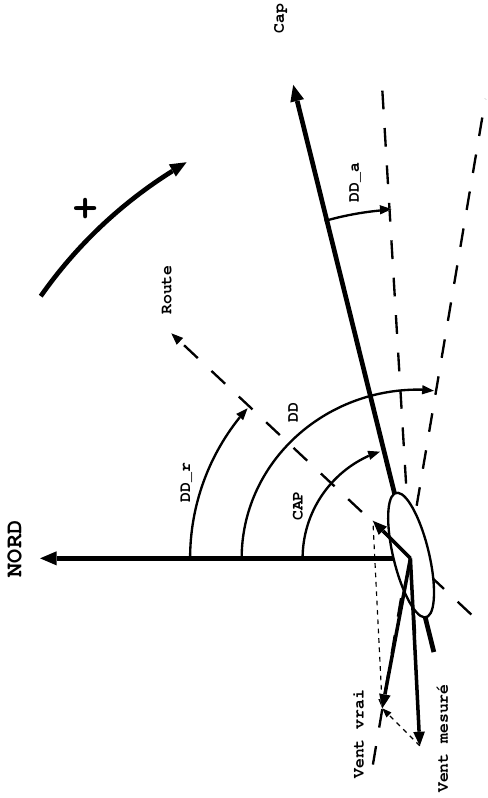
\includegraphics[angle=270,width=0.7\linewidth]{images/graph_arg_vent_bateau_polaire.png}
\end{center}

%%%%%AUTEUR%%%%
\itemstyle{Auteur~:}
CNRM/GMEI/TRAMM

%%%%%REFERENCE%%%%
\itemstyle{R\'ef\'erences~:}

